\subsection{Phases of matter}

An important area of research is the study of the different phases of (quantum) matter. A phase is a state of matter in which the macroscopic physical properties of the substance are uniform on a macroscopic length scale. These phases can be measured by the thermodynamic function, i.e.\ by a function of a few macroscopic parameters. \cite{Nishimori2011}. More precisely, for a given phase the properties vary as an analytic function of the macroscopic variables.
Interesting physics happens at the boundary between 2 or more distinct phases. The phase transitions were classified by Ehrenfest \cite{Jaeger1998}, who looked at the free energy across the phase boundary. If the free energy shows a discontinuity, it is called first order (or discontinuous) phase transition. Similarly, if the derivative shows a discontinuity, it is called second order (or continuous). Higher order phase transitions are possible, and there are even examples of infinite order transitions, such as the Berezinskii-kosterlitz-thouless (BKT) transition.  In 2016, kosterlitz and thouless were awarded the nobel prize in Physics for their discovery \cref{Bletenholz2016}.

\subsection{Symmetry breaking}

Sometimes, but not always, a phase transition is  related to spontaneous symmetry breaking. A state $\ket{\Psi}$ is said to be symmetric under a unitary transformation U if the state only changes by a phase factor: $ \hat{U} \ket{\Psi} = e^{i \phi} \ket{\Psi} $. A Hamiltonian possesses a symmetry if it commutes with U: $ [H,U]=0$  \cite{Beekman2019}. A remarkable fact is that many ground states are not invariant under a symmetry U of the Hamiltonian.
For phase transitions associated with a broken symmetry, one can define an order parameter. This parameter evaluates to 0 for the symmetric phase, but not for the spontaneous broken phase.
In continuous or second-order phase transitions the order parameter increases continuously from zero as the critical temperature is traversed. The entropy also changes continuously. On the other hand, the correlation length and related energy scales diverge at the critical temperature. In fact, at the critical temperature of a second-order phase transition, the system becomes scale-invariant, in the sense that physical properties no longer depend on the length (or energy) scale at which they are probed. Many symmetry-breaking phase transitions are second-order, with the onsets of superfluidity, (anti)ferromagnetism and many phases of liquid crystals as famous examples\cite{Beekman2019}.

\subsection{Universality}

Universality looks at the behaviour of the system near a continuous phase transition. These can be described well by so-called power laws. For classical phase transitions (driven by temperature) near the critical temperature $T_c$, observables $a_i$ depend in the following way on the reduced temperature $t=\frac{T-T_c}{T_c}$: $ a_i(t) \sim t^{\alpha_i}$ (see \cref{crit:cft}). One would expect that the set of critical exponents ${\alpha_i}$ depends on the precise form of the Hamiltonian of the system, but it turns out these exponents can be captured by a limited number of universality classes. This means that the physics near criticality is completely understood once it is understood for one member of the class.

\subsection{Critical exponents for spin systems}
\begin{table}[h!]
    \centering
    \caption{Definition of parameters for Ising model}
    \begin{tabular}{c c c c}
        Symbol & name                \\
        \hline
        m      & magnetisation       \\
        $\xi$  & correlation length  \\
        g      & external field      \\
        t      & reduced temperature \\
        $\tau$ & relaxation time     \\
    \end{tabular}
    \label{isingtable}
\end{table}

\begin{table}[h!]
    \centering
    \caption{Definition of parameters for Ising model. Values from \cite{Odor2004}.}
    \begin{tabular}{c c c c}
        Symbol  & relation             & 2D  value \\
        \hline
        $\beta$ & $m \sim t^{\beta} t$ & $1/8$     \\
        $\nu$   & $\xi \sim t^{-\nu}$  & 1         \\
        $z$     & $\tau = \xi^z$       & 1         \\
    \end{tabular}
    \label{isingtable2}
\end{table}

\Cref{isingtable} defines some parameters for the Ising system (see also \cref{models:ising}) and \cref{isingtable2} its relevant critical  exponents. The 2-point correlation function is defined as $ f( x,y) =  \left < m(x) m(y) \right > -  \left<m(x) \right> \left<m(y) \right> $. At larger distances this decays exponentially fast $ f(  x,y ) = e^{ -\frac{ |x-y|}{ \xi} } $ (see \cref{crit:cft}), where $\xi$ is the correlation length. For the ordered phase, the following relations hold: $m \sim |t|^{\beta} $ , $\xi(t) \approx |t|^{-\nu} $\cite{Odor2004}.  At the critical temperature near a quantum phase transition for 2D ising, the following relation holds: $ t \approx |g-g_c|^{z \nu_{3D}} $ \cite{Hesselmann2016}.

\subsection{Finite-size scaling}\label{subsec:fss}

Phase transitions only occur for systems with an infinite number of degrees of freedom. \cite{Kadanoff2010} This poses a problem, as in for instance Monte Carlo simulations only finite grids can be simulated. One computational expensive way to extract the properties in the thermodynamic limit is by making the grid increasingly bigger until the properties have converged. Fisher's  insight was that the properties could also be extrapolated from different finite-size calculations \cite{Fisher1967} by making the following assumption: near a critical point, every thermodynamic property scales as a universal function of $L/\xi$, with L the size of the system and $\xi$ the correlation length.
Define $t=\frac{T-T_c}{T_c}$. The mathematical formulation is \cite{Beach2005}
\begin{equation}\label{eq:fssansatz}
    A(T,L) = L^{\kappa / \nu} f_A( t L ^{1/ \nu} ).
\end{equation}
This holds for t small (near critical point) and L sufficient large compared to the lattice spacing. The exponents can be fitted by plotting $A(T,L)  L^{-\kappa / \nu} $ as a function of $t L ^{1/ \nu}$ for different sizes L and temperature t. For the correct critical exponents and critical temperature, all the points should collapse to one single graph. From the ansatz \cref{eq:fssansatz}, other ways can be derived to determine certain coefficients.

\subsubsection{Finite-size scaling for MPS}

The finite-size scaling for \Gls{MPS} is somewhat different. In \cite{Vanhecke2019}, it is argued that $\delta$ can take the place of $1/L$. Suppose $\lambda_i$ are the eigenvalues of \cref{vumps_transfer_eigs} ordered from the largest real part to smallest. Then
\begin{equation}
    \epsilon_i = - \log( \left | \lambda_i  \right |  )
\end{equation}
and
\begin{equation} \label{eq:cit_delta}
    \delta = - \sum_i c_i \epsilon_i  \quad \sum_i c_i = 0
\end{equation}
The intuition behind this is as follows: for an \Gls{MPS} approximation, the gaps in the transfer spectrum always go to zero for sufficiently large bond dimension. The distance between these gaps is thus a measure for the system size.

\subsubsection{Subleading corrections}
In \cite{Beach2005}, it is argued that the form proposed in \cref{eq:fssansatz} does also not fully take into account the finite-size effects. Subleading corrections could be introduced as follows:
\begin{equation}\label{ea:subleadparam}
    A(T,L) = L^{\kappa / \nu} ( 1+c L^{-\omega} ) f_A( t L ^{1/ \nu} -d L^{-\phi/\nu} )
\end{equation}
Indeed, this reduces to \cref{eq:fssansatz} for sufficiently large L. Because there is always data needed to perform the collapse in a region around the critical point, the original procedure could be biased and result in wrong parameters. On the other hand, introducing extra parameters can lead to overfitting, again not improving the result.

\subsection{CFT}\label{crit:cft}

One of the tools to derive some properties of phase transitions is Conformal Field Theory (CFT). CFT is a quantum field theory, which obeys an additional rule: the physics remains invariant under a conformal transformation. The exact form of these transformations is
\begin{equation}
    g'_{\mu \nu}(x') = \Lambda(x) g_{\mu \nu}(x) .
\end{equation}
In 2D, the shape of the correlation functions can be determined exactly, and indeed correspond to the form from the previous section. One of the properties characterising a conformal field theory is the central charge $c$, which can only take a discrete number of values.  In the case of unitary systems with $c \leq  1$, this has  turned out to give a complete classification of possible two-dimensional critical behaviour \cite{Ginsparg1988}. For the 2D Ising model, the central charge is $c=1/2$. A scaling relation used in the results chapter is \cite{Calabrese}
\begin{equation}
    L e^{  6 S( T,L ) /c }  \sim   \xi .
\end{equation}

\subsection{Quantum phase transitions}

A traditional second order phase transition is driven by a change in temperature. Quantum phase transitions on the other hand happen at zero temperature under influence of another parameter g of the model. At finite temperature, 2 things can happen (see \cref{fig:crit:qtran}): either there is a line connecting a classical second order phase transition to the quantum phase transition, or the phase transition disappears at finite temperatures \cite{Sachdev1999}.

\begin{figure}[h!]
    \center
    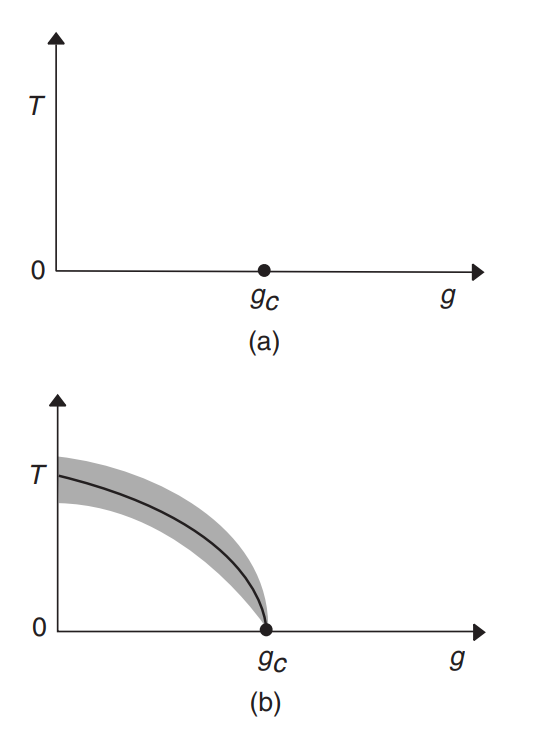
\includegraphics[width=0.5\textwidth]{Figuren/crit/Screenshot from 2021-05-06 15-58-55.png}
    \caption{ Two possible phase diagrams of a system near a quantum phase transition. In both cases there is a quantum critical point at $g = g_c$ and $T = 0$. In (b), there is a line of $T > 0$ second-order phase transitions terminating at the quantum critical point. The theory of phase transitions in classical systems driven by thermal fluctuations can be applied within the shaded region of (b).  Figure and caption taken from \cite{Sachdev1999}. }
    \label{fig:crit:qtran}
\end{figure}

